% !TEX root=frame_thesis.tex
\section{Methods and Model Description}

\begin{itemize}
	\item  General Idea of the Model
	\item Agents and Environment
	\item Setup Picture
	\item Discretised Map
	\item Modules
		\begin{itemize}
			\item Harvest 
			\item Happyness, Reproduction and Death
			\item Moving
			\item 
		\end{itemize}
	\item Sensitivity Analysis
\end{itemize}


\subsection{Overview of the Model}

%Topic: General overview of ABM
%Main Idea: Human agents interact with local Environment
In this thesis, I present an Agent Based Model (ABM) that simulates the settling of household agents on Easter Island and their interactions with the natural environment. 
This Easter Island environment is encoded on a 2D discretised map with specific real geographic features.
The agents rely both on a non- or slowly renewable resource, the palm trees, and a renewable resource, sweet potato cultivation. 
They gain access to these resources by cutting trees and occupying viable sites with agriculture gardens in their near surroundings, thereby relying on but at the same time changing their local environment.
Consequently, the household's population growth or decline depends on the success of this reosurce allocation. 
Furthermore, resource availability determines the settlement behaviour of the agents.
The interaction with the natural environment places constraints on the settlement patterns as well as population dyanmics of the overall Easter Island society.

%Topic: Time and Update Order
The model assumes yearly updates of the variables of each household agent and the environment throughout the time period of the prehistoric Easter Island society.
The simulation starts with the arrival of the first settlers at Anakena Beach in 800\, A.D.. 
All agents are updated in each timestep of one year in a random order. 
During the update of a single agent, the environment as well as the agent's features, like their population size and settlement location, are changed.
New household agents can appear following reproduction of existing agents throughout the simulation. 
The simulation ends in 1800 A.D. with the arrival of European voyages marking the latest end of the isolated status of the Easter Island society, since this presumably had a large impact on the society, e.g.\ through the introduction of diseases wiping out a large fraction of the Easter Island population in the 19th century.% \todo{cite Bahn2017}.

%Topic: I will describe the Model
In Section \ref{sec:CreateMap} I explain how I generate the 2D discretised map comprising the environment of Easter Island. In Section \ref{sec:AgentUpdate} I then focus on the household agents and updating a single agent.
This update is seperated into several modules: Calculation of the agents' Resource Needs, Tree Harvest, Agriculture Harvest, Reproduction and Death, and potentially Moving the settlement.
All of these processes and dependencies between them are explained in the following sections. Figure \ref{fig:SketchABM} summarises all environmental variables, the agent variables, and their dependencies.


\begin{figure}[H]
	\centering
	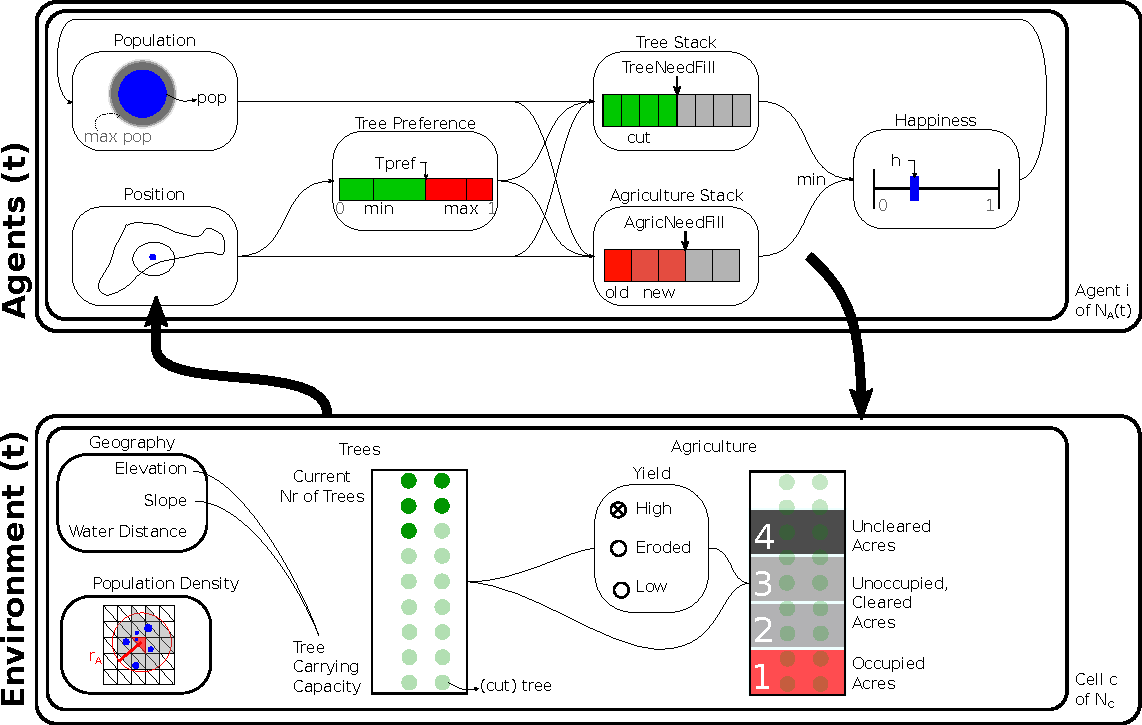
\includegraphics[width=1\textwidth]{images/SketchABM/SketchABM.pdf}
	\caption{A sketch of the presented ABM. At any time, agents have a population size, a settlement location, a tree preference, and corresponding tree and agriculture need. They try to fill this agriculture need by interacting with the environment's tree and agriculture modules. Finally, depending on the happiness the agent's population size is updated and settlement might be moved to a new location which is derived from the local environment.}
	\label{fig:SketchABM}
\end{figure}


\subsection{Creating a 2D discretised Map of Easter Island}

Before starting the simulation a triangularisation of a rectangular grid of points is created dividing the island into a number of small 2D triangular finite elements.
I use a 2D equidistant grid spannning from $-27.2050^\circ, \, -109.4650^\circ$ to $-27.0437^\circ, \, -109.2227^\circ$ and a resoultion of (i.e.\ $160$ points in $x$(East)- and $80$ points in $y$(North)-direction). 
In principle, the map can be created with any arbitrary resolution, constrained only by the resolution of the underlying geographical data. 
Also other grid types, e.g.\ one with higher resoultion at a specific region of interest, are completely compatible with the model. 
\todo{Why do i even get the problem of the weird triangles\ldots}
While higher resolution results in more detailed results, of course, computation time of the presented model scales highly non-linearly.
Hence, a trade-off has to be found between detail and computation time.
Given this grid, I use matplotlib's Delaunay triangulation tool to create 2D triangular finite elements.
The average area of such a triangle with the grid used in this thesis is \TODO.  
In summary, this approach produces a detailed map of Easter Island.

%Topic: Define Easter Island
Using geographical information, the triangles making up Easter Island are selected.
For this, I lay the discretised map over 2D elevation and slope maps obtained from Google Earth Engine (\TODO).
All triangles with midpoints situated on the ocean (i.e.\ elevation equals zero) are masked out and discarded.
The remaining triangles are considered part of the landmass of the simulated island. 
In the following these will be called cells.
With the resolution given above, $N_c = 11387$ cells remain. The area of the discretised map is $A=\TODO$, i.e.\ only a negligible fraction off from the $163.6\, {km^2}$ in reality.

% Topic: Cell 
A cell has several constant features (see Figure \ref{fig:SketchABM}):
First, geographic features of the cells are calculated.
A cell's location is defined by its midpoint. Since all cells are Delaunay triangles, the smallest angle is maximised. Hence, the midpoint provides a reasonable representation of the cell.
The features Elevation $el(c)$ and Slope $sl(c)$ of the cell $c$ are measured at this midpoint from the obtained maps.
There are three permanent crater lakes on Easter Island, providing the major freshwater sources for the prehistoric Easter Island population. Hence, the minimum distance $waterDist(c)$ of a cell to these sources is an important geographical feature.
Archaeological records indicate that crater lakes could have dried out during major drought periods.
In particular the drying of Rano Raraku in the East of Easter Island during the Medieval Climate Anomaly ($500-1200 \, \rm{A.D.}$) and during the Little Ice Age ($1570-1720\, \rm{A.D.}$) \citep{Rull2020} and the consequences have been a reoccuring theme of scientific debate (e.g.\ \citet{Cauwe2011}). 
Such drought events can be simulated by removing each of the lakes for some period of time from the map.

Second, biological features of the cells on Easter Island are derived. 
Each cell has an initial variable tree density. 
At the time of the arrival of the first settlers the islands forest system was in equilibrium (e.g.\ \citet{Brander1998}) except for possible climatic changes, which impacted tree cover \citep{Rull2020} but are not considered here. 
Therefore, the tree number on each cell constitutes a carrying capacity of palm trees for this cell. I assume this carrying capacity to be constant throughout the simulation.
There is is still a lot of uncertainty about the total number and patterns of palm trees at the time of arrival of the first settlers. 
\citet{MiethBork2015} estimate from root casts a total of $16\cdot10^6$ trees covering $80\%$ of the island, whereas \citet{Brandt2015} initialise the model with a conservative estimate of $8\cdot 10^6$ trees. 
Most studies assume an islandwide, dense distribution of the palm trees. 
E.g.\ \citet{Bahn2017} state that soil sufficient for tree growth is present `almost everywhere on the island, apart from the steepest parts of the cliffs and the youngest lava surfaces' (i.e.\ the highest elevations of Mount Terevaka). 
However, \citet{Rull2020} also investigates the possibility of mosaiic vegetation patterns with high densities of trees around the lakes and the coastal areas.
%As mentioned in the introduction \TODO, there's no comprehensive record of tree patterns. While some \todo{cite Rull?} archaeologsits state that the majority ($80\%$ of the island) was densley forrested \todo{cite}. 
The model presented here can incorporate any pattern of pre-arrival tree density. 
For the results in this thesis, I assume a pattern characterised by three geography-dependent tree density levels: (1) `normal density' for low elevation $el(c)<250\, \rm{m}$ and slope $sl(c)<5^\circ$, (2) `half density' for moderately high elevations $250\, \rm{m}el(c)<430\, \rm{m}$ (elevation of Lake Rano Aroi) and slope $5^\circ < sl(c) < 9^\circ$, and (3) `zero density' for cells above these thresholds.
$16\cdot 10^6$ trees are then distributed randomly to the cells according to this classification. 
In total, this produces a map (Figure \ref{fig:Map_tree}) with tree coverage of $80\%$ of Easter Island, representing the state of the forest at the time of the arrival of the first settlers.


The variabel tree density in each cell, $T(c,t)$, is decreased through the agents' deforestation throughout the simulation.
However, I also investigate a scenario with tree regeneration. After alteration by the agent's activity trees regrow logistically in each cell with the carrying capacity $T(c,0)$.
The growth rate (at $T(c,t)\ra 0$) of these trees is relatively slow and has been made responsible for the ecological degradation of the island according to some studies e.g.\ \citet{Brander1998}. 
\citet{Brandt2015} use values between $0.02$ and $0.07 \, \rm{1/yr}$ for their model.
In this model, experiments, in which tree regrowth is allowed, the logistic growth rate is $0.05\, \rm{1/yr}$. 
In some cells, trees are cleared out entirely in the simulation. 
I also want to allow for tree regrowth in such sites, which would see seeding e.g.\ from wind or birds or human activity.
Therefore, if a cell is completely barren, i.e.\ neither trees nor agriculture, for the $10$th years, a number of trees `pops up' ($0.5\%$ of the cell's carrying capacity).  
In the upcoming years these trees (if not harvested) grow logistically.
Since as described in the introduction, there is a large consensus that the Polynesian rats largely hindered tree regeneration by gnawing on the nuts (e.g.\ \citet{Hunt2007}, \citet{Bahn2017}), this tree regrowth is switched off in the standard setting of this model making the trees an entirely non-renewable resource. 
In order to investigate, the impact of this tree regrowth on the dynamics, experiments are performed with the process.

%Topic: Agriculture Yield
Easter Island's suitability for agriculture has been subject to excessive debate not least due to the first very contrary observations made by Roggeveen in 1722 as an `outstandingly fruitful' and by Cook in 1774 as an extremely poor and often sterile island \citep{Bahn2017}. %page 112   % who perceived the island's agricultural potential completely contrary \citep{Cauwe2011}.
Nevertheless, from archaeological studies we know that the Easter Island people cultivated sweet potato, taro, yam, banans, sugar cane and other crops.
Since sweet potato appears to be the dominant staple crop \citep{Louwagie2006}, I focus on this single crop here.
While the total potential of agriultural productivity remains uncertain, researchers identified viable sites and can distinguish between highly or less suitable land by using data on rain, climate, temperature, elevation and soil quality in agricultural models.
In this study, I use the map created by \citet{Puleston2017}(Fig 4) indicating sites that meet their climatic and soil quality criterion for being viable for sweet potato cultivation.
These sites are located mainly along the South, North East and West coast. 
Additionally, \citet{Puleston2017} indicate upland areas which do not meet the criteria but were nevertheless covered by patchy garden structures used by the Rapa Nui.
The authors calculate that this only adds a fraction to the overall agriculturally used land, though.
Throughout this study, I call the viable sites `high quality' and the upland gardens `low quality sites'.

\citet{Louwaried2006} also derives a criterion for successful cultivation of several crops based on climate and soil property measurements at several sites on the island. 
They found that, despite archaeological evidence for gardening in this area, one of the studied sites (Vaitea) was not suitable (with a relative yield of $0-20\%$ of an optimal site) for cultivation of the islanders main crops due to a lack of nutrient availability.
The islanders used techniques like lithic mulching on a large fraction of the island, which mainly reduced evapotranspiration and thus increased moisture availability, but also plant spacing and frequent fallowing.
This might have increased yields \citep{Louwarie2006}, but the per area harvest still remains low with these techniques in place.
This non-suitable site coincides with the upland low quality area defined by \citet{Puleston2017} (compare Figure 1 of \citet{Louwagie2006} with Figure 4 of \citet{Puleston2017}). 
The other sites in \citet{Louwaried2006} located at the foot of smaller craters along the South, North East and West coast were classified as mostly marginally to moderately suitable for sweet potato cultivation for most climatic conditions with some locations being highly suitable especially in wet years. 
They are mainly located in the high quality regions of the map in \citet{Pulestion2017}.
Again, through land management and labour intensive lithic mulching these yields could be enhanced, however the main limitation, nutrient availability, limits the success of such efforts. 
%{mention that lithic mulching mainly for water availabiliyt, but main limitation remains nutrient lack!!}
All in all, one can conclude that the expected yield of sweet potato farming strongly depends on the specific location and its climatic conditions and soil quality.
These complex processes alone require much more modelling and measuring research and so far have produced very different results with strong implications on the reconstructed history of the Rapa Nui.

In this model, I parametrise this complex process by using the map of high and low quality sites from \citet{Puleston2017} and assigning each cell to a relative yield of $100\%$ for high, $10\%$ for low quality sites and $0\%$ for non viable sites. 
However, the agricultural potential and its impact on the population carrying capacity of Easter Island remains a strong limitation in this model. %in estimating the carrying capacity.
The resulting map of Yields $Y(c)$ (shown in Figure \ref{fig:Map_agric}) gives \TODO $\rm{km^2}$ (i.e.\ $\TODO\%$) of high quality sites and, additionally, $\TODO\, \rm{km^2}$ (i.e.\ $\TODO\%$) in low quality sites.
%potential relative yield in the best class ($81-100\%$) but most locations were classified as marginally to moderate and  of the  coincide with either high or low quality sites 

As mentioned by some authors, soil erosion through radical deforestation and heavy rainfalls also constrain the agriculture potential of the island.
As trees are removed from the areas, rain can wash away fertile soil and leave less fertile ground with reduced yield \citet{Bahn2017} \TODO.
In the model I assume that, as a cell becomes completely treeless, soil yield of high quality sites is reduced to \TODO. 
This degradation is reverted as soon as trees pop back up, i.e.\ if the cell has been kept barren (withough agricultural production) for the past $10$ years.
\begin{figure}
	\centering
	\includegraphics[width=\textwidth]{images/Map_agric}
	\caption{A map of the potential agricultural yield of sweet potato cultivation in each cell of the discretised map of Easter Island. The map is obtained from \citet{Pulestion2017}. The relative yield of areas where gardening was observed but that did not meet the agricultural potential of \citet{Puleston2017}'s criterion is $10\%$ in line with the result of a model of agricultural yield from measurments in one such site by \citet{Louwagie2006}.}
	\label{fig:Map_agric}
\end{figure}

\subsection{Agents and Update Step}\label{sec:AgentUpdate}
% Topic: Agents Households with properties
The model simulates households represented as agents situated on the map.
%Agents have several constant properties: 
%A reproduction rate $rr$, a moving radius $r_M$, a resource search radius 
Agents have several variables describing their state.
Each agent $i$ is located on a position $(x_i,\, y_i)(t)$ on the discretised map and, hence, associated with one spefic cell $c_i(t)$.
The household consists of $pop_i(t)$ people, which can range from $6$ to $48$.
In order to sustain and potentially increase their population size, the agent relies on an intake of resources each year.
As described in the Introduction, I consider two major resources, tree cutting and sweet potato cultivation.
An agent can aquire these resources from cells within certain radii: The tree search radius $r_T$ and agriculture search radius $r_A$. 
I assume that both are fixed for all agents and throughout the simulation.
In each year, the agent searches for trees and if necessary new agriculturally viable sites in those cells, whose midpoints are within the search radius, $C_T(c_i(t))$ and $C_A(c_i(t))$, respectively.
\begin{eqnarray}
	C_{T/A}(c_i(t)) = { \tilde{c}\ | \ ||\text{midpoint of } \tilde{c}  - \vec2D{x_i,y_i}(t)|| \leq r_{T/A}}
\end{eqnarray}

However, this need for tree and agriculture harvest for each agent varies with the population size $pop_i(t)$ and an adaptive trait of the agent, the tree preference described in the following. 
In the initial phase, the islanders lived off the natural resources, i.e.\ birds, fish, and fruit from the trees \citet{Bahn2017}. 
Over time, the islander's economy `switched from predominantly hunter-gatherer to a dryland farming society' \citep{Louwagie2006}.
In this model this shift is reflected by a trait parameter of each agent, the tree preference $TPref_i(t)$, ranging from $0$ to $1$.
This tree preference indicates the value of tree harvest over agricultural production and, hence, increases the need for one over the other in order to fill the resource requirements.
The tree preference is high in the initial state, but decreases as trees become scarce and more land is available for cultivation of crops.
Hence, $TPref_i(t)$ responds to some degree to the local environment of the agent.
In this model, $TPref_i(t)$ depends on the local, relative change of tree density within the tree search radius $r_T$ with respect to the initial state:
\begin{equation}
	TPref_i(t) = f\left( \, \frac{\sum_{\tilde{c} \in C_{T}(c_i(t)) \, T(\tilde{c}, t)}}{\sum_{\tilde{c} \in C_{T}(c_i(t)) \, T(\tilde{c}, 0)} } \, \right)
\end{equation}
The shape of the function indicates a responsiveness of the economy/society to environmental change. How fast does the agent adapt its harvest requirements, when the non-renewable resource, trees, declines from the inital state?  
I am considering four possibilities: 
\begin{itemize}
\item The tree preference decreases linearly with the local, relative tree density decline (linear case).  
\item The tree preference decreases delayed with the local, relative tree density decline (delayed case).
\item The tree preference decreases quicker than the local, relative tree density decline (careful case).
\item The tree preference decreases first delayed, and at some point quicker than the local, relative tree density decline (switched case).
\end{itemize}
\begin{figure}
	\centering
	\includegraphics[width=\textwidth]{images/TreePreferenceOverTreeDensities}
	\caption{The relation of an agent's tree preference $TPref_i(t)$ adaption to relative changes in the local tree density for the four considered relationship types.}
	\label{fig:TPref_T}
\end{figure}
The tree preference is cut off at certain minmium and maximum thresholds, since an agent can hardly live off trees and its derivatives entirely and even for agricultural productivity a certain amount of trees is required (e.g.\ as cooking wood or for tools). 
I choose: $TPref_{min} = 0.2$ and $TPref_{max} = 0.8$, which is also the initial value for the first settlers.

In total, the agent's resource requirements of tree harvest, $TReq_i(t)$, and agricultural production, $AReq_i(t)$, per year are calculated as:
\begin{equation}
	TReq_i(t) = TPref_i(t) \cdot pop_i(t) \cdot TReq\_pP \, 
\end{equation}
and similarily, 
\begin{equation}
	AReq_i(t) = (1-TPref_i(t)) \cdot pop_i(t) \cdot AReq\_pP\, , 
\end{equation}
where $TReq\_pP$ is the tree requirement per year per person in absence of agriculture and $AReq\_pP$ is the required agriculture production per year in the absence of trees.
These parameters are crucial of course for the whole dynamics. 
For $TReq\_pP$, I am using an estimate of the model study in \citet{Brandt2015} (which had only half of the inital trees though). 
In the standard run I am using $5$ Trees per Person per year. However, I vary this parameter in a sensitivity analysis (see Section \ref{sec:SensitivityAnalysis}).
For $AReq\_pP$, I am using the estimates by \citet{Puleston2017}. In their agricultural model, they identify the Nitrogen fixation as a major uncertainty in the evaluation of potential agricultural yields. 
With two different assumptions of Nitrogen fixation in the soil (high and low), \citet{Puleston2017} model the sweet potato harvest on a high quality agriculture site and combine it with the nutritional need of an individual person.
I do not consider fallowing in the model, as this in general reduces the per area harvest (while its higher effectiveness decreases the labour for a single worker), since I focus on map constraints rather than modelling labour. \todo{Check this statement}.
One can then calculate that for high N-fixation for one person (in the abesence of other food} needs $0.5\, \rm{acres}$ of high quality agricultural productivity of sweet potato cultivation.
In the case of low N-fixation this increase to $1.7\, \rm{acres}$ per Person. 
Here, I am using both values in order to test the different scenarios.
The resource requirements for trees given in absolute numbers and agricultural production given in acres of high quality agriculture sites are thus agent-specific features updated each year, which can be tuned through the global parameters $TReq\_pP$ and $AReq\_pP$.

% Topic: Fishing Agents constrained by a tabu 
The model allows for open sea fishing as a replacement for the agricultural requirement, for some agents living near the coast of Anakena.
%Instead of filling the agricultural requirement by cultivating land with crops, these deep-sea fishing household agents obtain their nutrition from the sea in the model. 
For such fishing agents, the agriculture and tree requirement are calculated in the same way. However instead of occupying land units and harvesting agriculture, like other agents, fishers simply fill this requirement by going out to sea. 
In the initial phase of Easter Island settlement, fish supply was plentiful, with excarvations proving that shellfish, fish and even porpoise like dolphins were a major part of the diet at the time \citep{Bahn2017}
However, over time, this resource became more and more scarce and many species even went extinct due to human predation. 
From \TODO we know that as a reaction to this development the Easter Island society introduced a taboo on fishing. 
Only members of a specific chiefdom living at Anakena Beach could pursue it \todo{cite}. 
According to \citet{Bahn2017} or \citet{Diamond2005}, sea fish vanished from the Easter Island typical diet by \TODO.
Hence, in the model, every agent living within $r_A$ distance of Anakena Beach becomes a fishing agent.
At time $t_\text{taboo fishing}=\TODO$ a taboo is put in place letting only \TODO those agents already pursuing fishing to continue but allowing no further agents to enter this resource stock. 
While I assume that fish supply is unlimited, another constraint of course is the tree requirement, which is quite extensive for building the canoes or providing firewood. Hence, the fisher's minimum tree Preference is set to $TPref_\rm{min}|_\text{fisher} = 50\%$ rather than $TPref_{\rm{min}} = 20\%$ for agricultural agents.
While agents, that are allowed to fish, do not have any agricultural requirements due to the assumed unlimited resource stock from the sea, the correspondingly higher requirement for trees still needs to be fulfilled.

\subsection{Agent-Environment Interaction -- Tree and Agriculture Harvest}\label{sec:Harvest}
\begin{itemize}
	\item Tree Harvest
	\item Agriculture harvest
	\item How many trees to burn
	\item Fishing 
\end{itemize}

% Topic: Tree Harvest
After calculating the requirements of tree harvest and agricultural production as described in the previouse section, an agent tries to fill these.

By occupying land units of $1\, \text{acre}$ an agent increases their agricultural Production $AProd_i(t)$ in order to fill the agricultural requirement $AReq_i(t)$.
The occupied sites by agent $i$ are denoted as $acres_i(t)$, where each element is associated with one cell ($c(a)$ for $a \in acres_i(t)$) and the production obtained from these is:
\begin{equation}
	AProd_i (t) = \sum_{a \, \in \, acres_i(t)} \, Y(c(a))
	\label{AProd}
\end{equation}
The agent increases $AProd_i(t)$ by occupying more sites and adding them to $acres_i(t)$ until there are no further sites available or the requirement $AProd_i(t) \geq ARequ_i(t)$ is fulfilled.

An agent first searches for acres in cells with a potential for high quality sites ($Y(c)=1$), to minimise the workload.
An acre in such a cell can only be occupied (or added to $acres_i(t)$) if at least the necessary space is cleared off trees. 
Assuming that the trees are evenly distributed on the cell's area, the condition can be calculated as 
\begin{equation}
	\text{Treeless Area\,[acre]} - \text{Occupied Acres\,[acre]}  = 
	\left( 1 - \frac{T(c,t)}{T(c,0)} \right) \cdot \text{Area}(c) - \text{Occupied Acres}(c) geq 1
	\label{eq:BurningCond}
\end{equation}
If there are no high quality sites left that fulfill this condition, the agent uses the slash and burn method to reduce the number of trees $T(c,t)$ for the cell $c$ where the least amount of trees need to be burned until the condition holds.
The use of fires to clear space is supported by the extensive charcoal record starting with the period of intensified agriculture \citep{Mieth2015}. 
However it is not clear whether trees were felled and used (e.g.\ for extraction of the sugar sap) before burning and consequent agricultural use of the land \citep{Mieth2015} or slash and burn method was used directly to clear space (e.g.\ indicated by \citet{Bahn2017}). % Bahn: ``fires directly accompanied by agriculture''
If after occupying all available high quality sites the requirement is not yet fulfilled, i.e.\ $AProd_i(t)<AReq_i(t)$, the agent also considers low quality sites in the same procedure.
The agent keeps all occupied sites $acres_i(t)$ until the next year.%, i.e.\ $acres_i(t+1) = acres_i(t) + new\_acres(t+1)$.
New sites are, thus, only occupied in the model if the agricultural requirement has increased from last year through population growth or tree preference decrease or if the soil quality of occupied sites has degraded through erosion compared to the previous year.

After filling the agricultural requirement, the agent then cuts trees in order to fill the tree requirement. 
An agent selects random cells from $C_T(c)$ with probabilites proportional to the tree number $T(c,t)$ on them.
Then, the agent removes one tree successively from these cells and adds these to $TCut_i(t)$.
This is done successively until its tree requirement is fulfilled, i.e.\ $TCut_i(t)=TRequ_i(t)$, or there are no trees left in cells within the $r_T$ distance of the agent.
Unlike the agricultural production, where occupied sites are kept and re-used (with the same yield) in the next update, the agent needs to find new trees every year, i.e.\ $TCut_i(t)$ is starts at $0$ each year.
If tree regrowth is switched off, this tree harvest therefore represents a non-renewable resource dependency.

Figure \TODO \ref{fig:treeburning} shows an example sketch of potential procedure of deforestation and consequent replacement by agriculture in an example cell. 

\begin{figure}
	\centering
	\includegraphics[width=\textwidth]{images/sketchDeforestation.png}
	\caption{Sketch of deforestation procedure in an example cell $c$ (box). 
		In the beginning the cell has 17 of its initial 20 trees still standing. 
		The area of cell $c$ is $3.2\, \rm{acres}$. 
		Agent $a$ removes 5 trees from cell $c$ (among others potentially) to fulfill its tree requirement. An agent $b$ consequently occupies the now free space on cell $c$ for agricultural production. 
		Next, an agent $c$, needs to occupy more sites to fill its agricultural requirement as well and cannot find any other unoccupied acre in $C_A(c_c)$ despite the ones in cell $c$. 
	However the agent needs to burn $5$ trees before being able to occupy the second acre on this cell.}
	\label{fig:treeburning}
\end{figure}

Each year the agent tries to fill its requirements for trees and agriculture as much as possible with the procedure described above. 
Afterwards I evaluate the happiness $h_i(t)$ of this agent, reflecting the success of the harvest.
Assuming that filling the tree requirement and the agriculture requirement is equally important to the agent, the happiness is simly the minimum of the fraction of requirements that could be filled:
\begin{equation} 
	h_i(t) = min \left( \frac{TCur_{i}(t)}{TRequ_i(t)}, \, \frac{AProd_i(t)}{AReq_i(t)} \right)
	\label{eq:h_i}
\end{equation}
If both requirements are filled for agent $i$, $h_i(t)=1$.
However, if there either $TCut_i(t)$ or $AProd_i(t)$ are $0$, $h_i(t)=0$ regardless of the success of filling the other requirement.
Since agent's usually have some inertia in reacting to changes in harvest success (e.g.\ by storing some food over the years), I furthermore calculate a smoothed happiness $H_i(t)$:
\begin{equation}
	H_i(t) = \frac{h_i(t) + h_i(t-1)}{2}
\end{equation}
This factor also ensures, that if the agent has constantly too few resources, the happiness will decrease monotonically.
This happiness and smoothed happiness, as indicators of how well the agent is doing, determine responses to the harvest year (Reproduction, Population decline, or Moving the Settlement), which are described in the following section.


\subsection{Agent's reaction to the harvest}\label{sec:Reaction} 
\subsubsection{Population Dynamics}

%The population of an agent is assumed to b

After agricultural production and tree cutting, the agent's population size is adapted. 
The growth rate (positive or negative) of the agent's population at a specific time depends only on the smoothed happiness. 
\begin{equation}\label{eq:popgrowthcontinuos}
	pop_i(t+1) = g(H) \cdot pop_i(t)
\end{equation}
In fact, instead of assuming continuous growth or decline according to this growth rate, I consider a discrete, stochastic version of this.
Each individual memeber of the agent has a $1-g(H)$ probability to di, if $g(H)<1$, or a $g(H)-1$ chance to reproduce (i.e.\ adding one individual to the household/agent), if $g(H)>1$.
The population size stays constant at $g(H)=1$. 
This results in a stochastic growth/decline of the population where each agent's course is a realisation that can vary. 
Figure \ref{fig:app:PopulationGrowth} \TODO in the appendix shows a few different realisations of such a growth scenario with constant growth rate $g=1.007$ in comparison with the continuous growth.
The expected trajectory, though, follows the continuous growth from equation \ref{eq:popgrowthcontinuos} (compare e.g.\ with \cite{Bungartz2013}).

The reproduction rate of the Easter Island population in the case of unlimited food supply, i.e.\ especially in the initial phase, is quite widely discussed in the literature.
Parameters used range from $0.7\%$ per year \citep{Bahn2017} or `always below $1\%$' \citep{Brander1998} to exceeding $3\%$ for short periods of time or even $2.3-4.5\%$ \citep{Brandt2015}.
It is clear that depending on the story and proposed chronology, researchers have to make very contrary assumptions on the population growth in order to fit the few undisputed facts about population dynamics on Easter Island. 
If an arrival around 1200 is assumed (as in \citet{Hunt2007} or \citet{Brandt2015}), assuming a large population growth is unavoidable. 
There is no way, that only a few hundred inhabitants in the 14th and 15th century could have caused a massive alteration of the island's environment and created several hundred Moai.
With most researchers proposing arrival dates around 800, one has more freedom in choosing the initial growth rate, especially considering that there might have been several phases of population declines as proposed in \citet{\TODO Bahn2017}. 
One could imagine that after initial fast growth of the population after an early arrival, through fertility control a steady population size was reached below Easter Island's resource carrying capacity. 
Archaeological and charcoal data, however, suggest an intensification of human activity (and its impacts on the environment) only at around 1200 \citet{Hunt2007} and very little environmental impact before that.
Most researchers rather assume a slow but continued population growth from an early arrival to a peak population around 1300-1700 (e.g.\ \citet{Brander1998}, \citet{Bahn2017})
Hence, choosing an early arrival date here ($t_0=800\, A.D.$), I assume a slow growth rate in case of unlimited food supply and, therefore, happy agents: $g(1)=1.007$.

The specific dependency of the population growth/decline with limited food resources is another uncertainty.
\citet{Lee2008} have constructed a food-limited dempgraphy model which was applied for the Polynesian context \citet{Puleston2008} and extended and to Easter Island society and agricultural constraints in \citet{Puleston2017}. 
Here I take a very simplified result of this model to parametrise the impact of non-optimal harvests on the population dynamics. 
The model calculates age-dependent survival and fertility rates, which are both S-shaped curves w.r.t.\ the food availability, i.e.\ high for large food availability and low for scarce food availability.
Since, I do not consider structures below the agent/household level, I simply assume a growth rate with the same shape as the survival and fertility rates.
\begin{equation}
	g(H) \sim CDF(\Gamma_\text{Dist}(shape, scale=0.1))
\end{equation}
where $CDF(\Gamma_\text{Dist})$ is the cummulative density function of the Gamma distribution with scale set as in \citet{Lee2008}.
I then tune the shape parameter of this function to give the same equilibrium point $g(H)=1$, i.e.\ a constant population size, as in \citet{Puleston2017}: $g(H=0.6883)=1$. 
In order to test sensitivity of this parameter, I also investigae a higher shape parameter $shape=3$\TODO, which leads to a less resilient population size as resource scarcity sets in: $g(H=0.84)=1$ and steeper decline of $g$ for $H<1$.
The amplitude of the resulting function is scaled to give the chosen reproduction rate under unconstrained food supply from the last paragraph: $g(H=1)=1.007$.
Figure \ref{fig:growthrate} shows the resulting dependence of the growth/decline rate of a household $g$ on the smoothed happiness $H$ (for the standard run in blue and a less resilient case in red for testing the sensitivity).
\begin{figure}[
	\centering
	\includegraphics[width=\textwidth]{images/reproductionrate}
	\caption{}
	\label{fig:growthrate}
\end{figure}
At $H=1$, the households population grows with rate $1.007$, as tree or agricultural land availability decreases, the agent's smoothed happiness decreases and so does the growth rate. If $H<0.6883$, the population size decreases.
If the household size $pop_i$ of an agent $i$ falls below a certain threshold $pop\_min = 6$, the agent $i$ disappears and the remaining individuals are adopted by other households living within $C_T(c_i)$ and are chosen randomly. \TODO
It should be noted, that the use of the model in \citet{Pulestion2017} is strongly simplified here.
E.g.\ I am using a different notion of food/tree availability, which I express via the smoothed Happiness, rather than \citet{Puleston2017}'s food requirement.
Also the distinction between survival and fertility rate especially given their age-dependency is entirely neglected.
Nevertheless, the resulting dependency of growth/decline rate on the agent's happiness (and consequently its success in resource acquisition) given in Figure \ref{fig:growthrate} is reasonable. 


\begin{itemize}
	\item Reproduction
	\item Population Shock
\end{itemize} 
 \subsubsection{Moving the settlement}
\begin{itemize}
	\item Moving according to penalties
\end{itemize}



% TODO: Measure Agric Productivity in acres of high quality sites
% TODO Why Wood is a primary resource
% TODO Tree Pref changes quickly
% Mention non-reneqabl etc. earlier.
% TODO Burning not really sure??

